\chapter[Toolchain Development]{Toolchain Development\footnote{A version of this chapter has been accepted for publication at the 2012 IEEE International Conference on Humanoid Robots \cite{ChoudhuryHumanoids2012}}} % (fold)
\label{cha:toolchain}

This chapter introduces a rapid prototyping toolchain\footnote{This work was completed in collaboration with Quanser Inc through the Natural Sciences and Engineering Research Council (NSERC)'s Industrial Postgraduate Scholarship Program.} developed to streamline the process of exporting a prototype design from a Computer-Aided Design (CAD) software package to generate dynamic simulations with full 3D visualization. Starting from the initial prototype design and drivetrain specifications in the previous chapter, the design process outlined in Section~\ref{sec:design_process} is used to improve the overall system performance. The toolchain provides an automated two-step process which begins by exporting key information from CAD (Section~\ref{sec:cad_export}) and ends by regenerating the equivalent system in a simulation environment (Section~\ref{sec:model_generation}). A case study is presented in Section~\ref{sec:case_study} demonstrating the performance benefits of the proposed toolset. 

\section{Design Process} % (fold)
\label{sec:design_process}

The electromechanical design and development of multibody robotic systems is an iterative process, starting from a mechanical model in CAD software, transferring its parameters to a dynamic simulator for analysis and revising the design to improve the performance of the system. This process is repeated until the mechanical design achieves some desired goal. The iterative nature of the design and analysis process can often become time consuming and cumbersome. However, for high DOF multibody systems, the iterative approach is necessary as small changes in the mechanical design can have a significant impact on the overall dynamics of the system and the resulting system behaviour as well as implications for control design. Another popular approach is the use of optimization tools \cite{Paul2001,Wollherr2002} to determine the optimum design configuration. However, the resulting configuration may not be realizable with the available hardware components and must still be verified in simulation before hardware implementation. 

There exists a wide variety of dynamic simulation environments with a range of capabilities \cite{Koenig04designand,michel2004webotstm, Kanehiro:2004dq, PonticelliCWR2006, Reichenbach2009, MedranoCerda2010}. These environments provide a feature complete package, which combine an underlying dynamics engine with an interface for visualizing the simulations. The underlying computation engines obtain the complete equations of motion for the system described by its kinematic/dynamic parameters using techniques including, but not limited to, Lagrange multipliers \cite{Baraff1996}, Kane's method \cite{Rosenthal1986} and port-based modeling \cite{Paredis2001}. The equations of motion are integrated to obtain the system state at each time step. Most simulators provide support for importing common Virtual Reality Markup Language (VRML) or Standard Tessellation Library (STL) files generated by CAD tools for visualization \cite{Koenig04designand,michel2004webotstm}. However, only a few provide direct compatibility with CAD tools to import kinematic/dynamic parameters for simulation.

Open Architecture Humanoid Robotics Platform (OpenHRP) \cite{Kanehiro:2004dq} is a commonly used dynamic simulation environment for humanoid robots that supports importing VRML files. However, kinematic and dynamic parameters of the robot are specified as plain text, making it cumbersome for rapid iterations.

MapleSim \cite{sw:maplesim} is a multibody simulation package that provides limited functionality to communicate with CAD applications through its MapleSimConnector toolbox. This toolbox uses the underlying Maple engine with command-line access for retrieving the parameters of each link. However, the CAD application has to be actively running in the background and it is left to the user to generate Maple worksheets for batch importing of the parameters to update the link parameters in MapleSim through its API.

SimMechanics \cite{sw:simmech} provides mechanical import functionality to generate Extensible Markup Language (XML) files containing link parameters directly from CAD along with the corresponding STL files for visualization. However, there are limitations on how joint constraints are defined in CAD to successfully generate an equivalent model in Simulink. Another drawback of this approach is that the visualization generated during simulations significantly impacts the simulation speed.
% section design_process (end)

\section{CAD Export} % (fold)
\label{sec:cad_export}

An add-in was developed for CAD software package SolidWorks to export a multibody system for dynamic simulations in Simulink with realtime visualization. Consider a standard multibody system with $n$ joints and $n + 1$ links. The links are numbered from 0 (base) to $n$ and each $joint_{i}$ connects $link_{i-1}$ to $link_{i}$. The mechanical design of each link is represented by its own CAD assembly (or part) file. The coordinate system at the origin of this CAD file is treated as the local coordinate system $xyz_{i}$ rigidly attached to the link $i$. The top most CAD assembly (referred to as the \emph{master assembly}) contains all $n + 1$ links as subassembly files connected and constrained by the mechanical relationship which defines the behaviour of each joint $n$. For example, a revolute joint connecting two link subassemblies is defined by the appropriate constraints (i.e. concentric relationship).

\begin{figure}[!h]
	\centering
    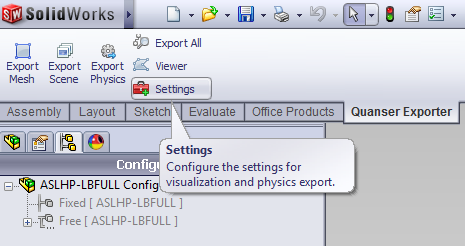
\includegraphics[scale=1.0]{fig/ch3/exporter.png}
  	\caption{The exporter add-in for SolidWorks (named Quanser Exporter in the SolidWorks tab) to capture relevant physical and visualization data.}
	\label{fig:swexporter}
\end{figure}

The add-in for SolidWorks uses this master assembly file as a starting point to export the multibody system for dynamic simulations. Once installed, a new tab is added directly in SolidWorks (as shown in Figure~\ref{fig:swexporter}) presenting the user with several export options. The initial export process prompts the user with a flat list of all subassemblies in the current file via a \emph{Model Organizer} interface (shown in Figure~\ref{fig:modelorg}). Each subassembly is treated as a node that can be ordered (through a drag-and-drop interface) to form the desired kinematic tree/chain hierarchy. 


\begin{figure}[!h]
	\centering
    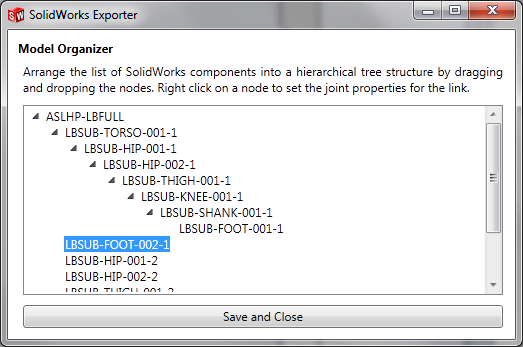
\includegraphics[scale=1.0]{fig/ch3/modelorg.png}
  	\caption{The \emph{Model Organizer} window used to define the kinematic structure of the system during initial export.}
	\label{fig:modelorg}
\end{figure}

\subsection{Physics Export} % (fold)
\label{sub:physics_export}
Each link subassembly is parsed in the order defined in the \emph{Model Organizer} window to extract key kinematic/dynamic parameters. All numerical values (i.e. distance between links) are extracted directly using CAD tools. Assuming that the system is in the home configuration at the time of export, the relative frame transformations $T^{i-1}_{i}$  between subsequent frames are extracted in accordance with the kinematic hierarchy defined in the \emph{Model Organizer}. The absolute frame transformations $T^{0}_{i}$ are also computed with respect to the base link (if the base link is fixed in the master assembly file). For floating base systems (i.e. base link has 6 DOF), the absolute frame transformations $T^{W}_{i}$ are taken with respect to the coordinate system of the master assembly file (world frame). The mass and dynamic properties are extracted with internal CAD tools in the local coordinate system of the link subassembly file. The mass, distance to the center of mass (COM) and inertia tensor of the link (at the COM position) are extracted.

The add-in captures these key parameters and generates a structured XML file. A XML node is generated for each link containing the extracted kinematic/dynamic parameters (as shown in Figure \ref{fig:exportfile}). Furthermore, each XML link node is organized in accordance with the kinematic hierarchy of the system. As a result, the add-in captures the entire physical description of the multibody system in a portable, language independent file.

\begin{figure}[!h]
	\centering
    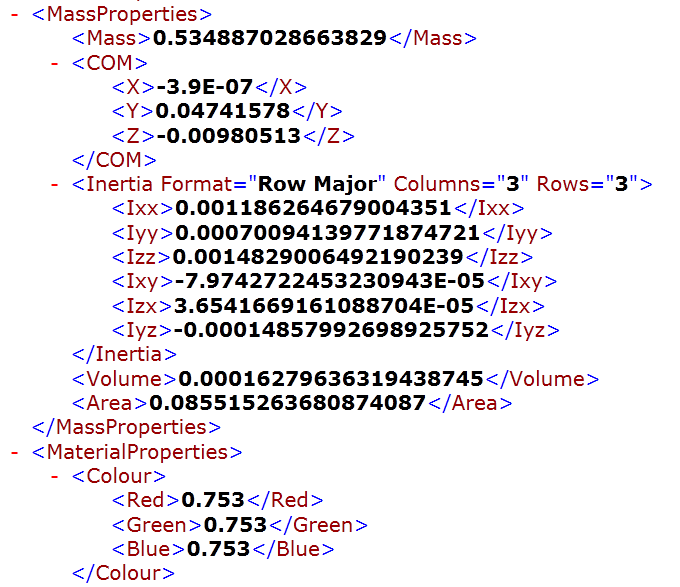
\includegraphics[scale=0.6]{fig/ch3/exportfile.png}
  	\caption{Example of kinematic and dynamic parameter extraction straight from CAD model stored in the exported XML file.}
	\label{fig:exportfile}
\end{figure}

% subsection physics_export (end)

\subsection{Mesh/Scene Export} % (fold)
\label{sub:mesh_scene_export}
In addition to exporting the physical description of the model, the exporter add-in also generates files for visualization. These files can be used in conjunction with dynamic simulations to provide the user with visual feedback of the system under control. Some dynamic simulators (SimMechanics, MapleSim) currently allow users to specify a VRML file for each link of the multibody system. While SolidWorks currently has some support to export VRML files for each link subassembly individually, there are no options to generate the 3D meshes in X3D format (successor to VRML).

The toolchain provides automatic batch generation of full 3D meshes in the X3D format for each link subassembly. Once the export process has been initiated, the meshes are extracted for each link subassembly in the master assembly file directly from the CAD layout. Each mesh is aligned with the local coordinate system of the link such that there is a direct mapping between the visualization and the physical model.

\begin{figure}[!h]
	\centering
    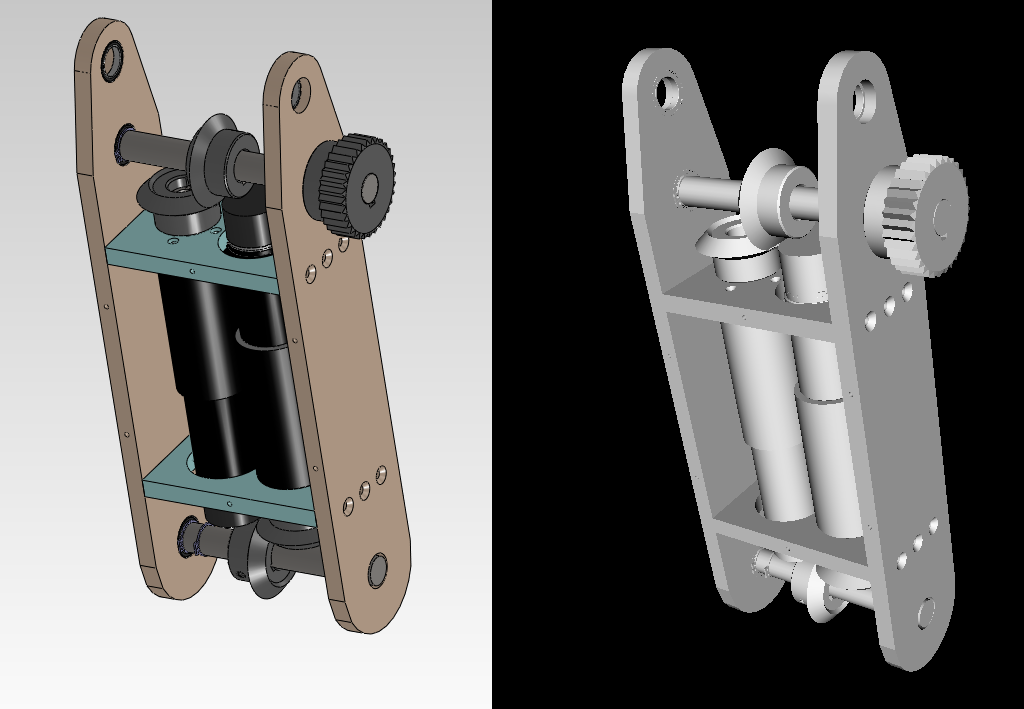
\includegraphics[scale=0.5]{fig/ch3/cad2x3d.png}
  	\caption{Equivalent X3D mesh file generated directly from CAD layout for a single link subassembly.}
	\label{fig:visualcom}
\end{figure}

The overall mesh generation process is optimized for complex multibody systems. A typical CAD subassembly representing each link may contain hundreds of smaller CAD part/assembly files. During the mesh generation process the add-in creates a new flattened version of each link subassembly and discards any visual details not visible on the surface. The surfaces of this flattened model are tessellated to generate the mesh file for each link. As a result, the mesh files are light weight and this helps speed up the rendering process.

The output mesh files are stored in the same directory as the XML file containing the physical description of the system. Furthermore, each link XML node is also updated with a complete path to its corresponding mesh file alongside the kinematic/dynamic parameters. The add-in also generates a \emph{scene} file from the CAD master assembly. This is a parallel XML file which contains a complete visual description of the system from CAD. The scene file contains a list of all links alongside their corresponding mesh files. These meshes are then organized in accordance with the kinematic tree/chain hierarchy provided by the user in the \emph{Model Organizer}.

As a result, the scene file recreates the visual layout of the complete multibody system from the CAD master assembly file. This file encapsulates the full multibody system in a format which is compatible with the 3D visualization blocks that are packaged with the QUARC toolbox. In addition to the model itself, additional supplementary mesh files (i.e. ground plane) are imported into the scene for visualizing the environment.
% subsection mesh_and_scene_export (end)

\subsection{CAD Update} % (fold)
\label{sub:cad_update}
With minimal user input, the add-in captures a complete physical and visual description of the system in its \emph{current state}. However, the main benefits of this toolchain becomes apparent after the initial export. Once the user defines the structure of the system (kinematic hierarchy and joint definitions) through the \emph{Model Organizer}, it is stored in memory for later use. Subsequent updates to the CAD model can be exported with a single click if the overall structure of the links and joint definitions do not change.

This allows the user to export a model for simulation from CAD, analyze the behaviour of the system under control, tweak the mechanical design and immediately re-export the revised model for simulation. For example, increasing the length of a link may alter its dynamic properties  while the overall kinematic structure remains the same. The revised CAD model with increased link length can be exported with a single click. The export process simply recalls the structure of the system and regenerates the XML files with updated kinematic/dynamic properties. The add-in also allows the user to regenerate only the mesh file for the updated link to reflect the changes in CAD. This process makes it fast and easy for rapid iterations during the design phase.
% subsection cad_update (end)

% section cad_export (end)

\section{Model Generation} % (fold)
\label{sec:model_generation}

The XML files exported by the add-in encapsulate the relevant information which describes the CAD model into structured and portable files. One of the key advantages of this approach is that the information in these files can easily be parsed to generate an equivalent model in most dynamic simulators. A model generation counterpart was developed for the Matlab/Simulink environment which uses SimMechanics for multibody dynamic simulation and Quanser's QUARC toolbox for 3D visualization. This provides a semi-automated toolchain for designing robotics and/or mechatronic systems.

The model generation approach provides several Matlab functions, scripts and libraries to parse the files exported by the SolidWorks add-in and generate the equivalent mechanical system in Simulink. The generated Simulink model contains (a) SimMechanics blocks with the link kinematic and dynamic parameters from CAD and (b) visualization blocks from QUARC libraries with the link meshes and scene file. The generated physics and visualization counterpart is prepopulated with CAD data and connected according to the kinematic hierarchy of the system defined in the \emph{Model Organizer}.

The model generation process is initiated by calling a function in the Matlab terminal inside the CAD export folder. By default, this approach generates a physical subsystem (i.e. the “plant”) for forward dynamics simulation, whose output drives a generated visualization subsystem. The user can also generate an inverse dynamics model through the command line.

\subsection{Physical Model} % (fold)
\label{sub:physical_model}

The physical model generation process parses the XML output files in the export folder to create a CAD-equivalent system in Simulink. In order to streamline the process, a library of masked link subsystems representing common link configurations (shown in Figure \ref{fig:quarcmech}) was developed. Each of these subsystems contains a combination of SimMechanics joint, body, actuator and sensor blocks to represent a combination of $joint_{i}$ and $link_{i}$ (shown in Figure \ref{fig:undermask}).

\begin{figure}[!h]
	\centering
    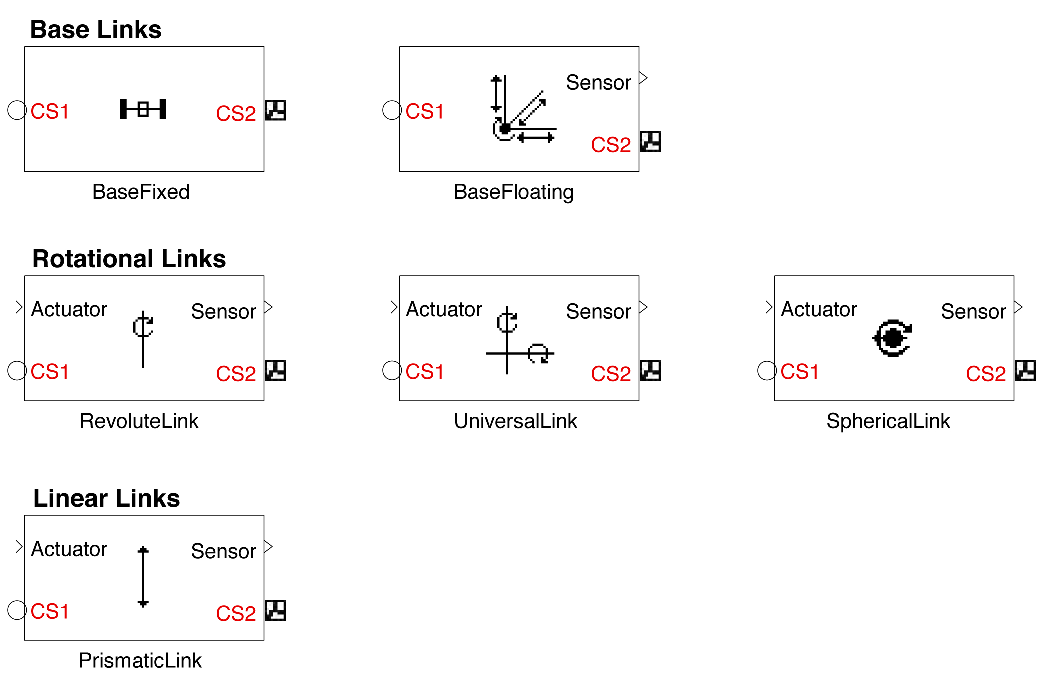
\includegraphics[scale=0.75]{fig/ch3/simmech.pdf}
  	\caption{The standard link subsystems for physical model generation with prepopulated kinematic and dynamic parameters from CAD.}
	\label{fig:quarcmech}
\end{figure}

The input to each link subsystem (\textbf{CS1}) is a connection from $link_{i-1}$ and the driving signal for the joint. The output of the link subsystem is its local coordinate system (\textbf{CS2}) and the joint sensor signals. The joint actuator/sensor signals are set depending on the type of dynamic simulation. By default the model generation process configures the physical model in forward dynamics mode so the joint actuator port is connected to the force/torque command input for $joint_{i}$ and joint angle/displacement is measured at the output. Alternatively, for the inverse dynamics simulation, the joint acceleration is set as the input, while the joint force/torque is the output. The output coordinate system of the $joint_{i}$ block is connected to a SimMechanics body block representing $link_{i}$. The masked parameters are preconfigured to set the local dynamic properties (i.e. COM position, inertia tensor) and relative frame transformation appropriately.

\begin{figure}[!h]
	\centering
    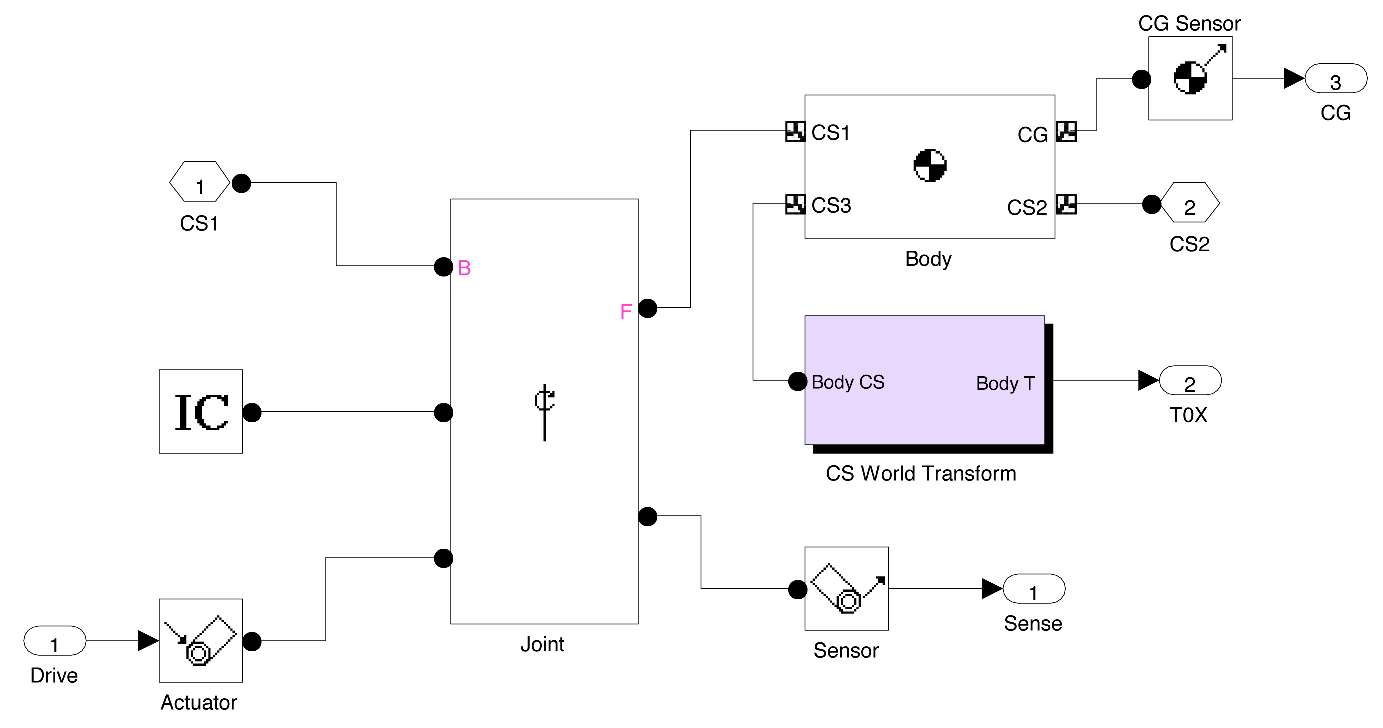
\includegraphics[scale=0.6]{fig/ch3/undermask.pdf}
  	\caption{SimMechanics blocks used to compose each CAD-equivalent link subassembly in Simulink}
	\label{fig:undermask}
\end{figure}

Each link subassembly from CAD is recreated with a link subsystem from the library depending on the link type. The masked parameters are populated with the kinematic and dynamic parameters from the corresponding XML link node. The overall hierarchy of links is parsed and each link subsystem is connected accordingly. The model generation process also automatically handles the signal routing from the input/output ports of the physical model. In the default forward dynamics configuration, the $n \times 1$ torque/force vector is connected to all joint actuator blocks and the output signals from the sensors are also routed accordingly. For the inverse dynamics case, the vector of joint positions, velocities and accelerations are connected to the joint actuator blocks and the sensors are preconfigured to output the resulting torque/force vector.

In addition to the link subsystem, a ground block representing the coordinate frame of the CAD master assembly is connected to the base $link_{0}$. The entire process of creating an equivalent model for dynamic simulation is automated. The user simply calls the appropriate function and the generated physical model subsystem is placed in a new (or existing) Simulink diagram.
% subsection physical_model (end)

\subsection{Visualization Model} % (fold)
\label{sub:visualization_model}
The visualization model generation process generates a single subsystem containing blocks to initialize and drive the scene file generated from CAD. The mesh for each link in the kinematic chain is driven by the output of the generated physical model (forward dynamics subsystem) so that there is a 1:1 mapping between the plant and what is being rendered by the visualization. When a simulation is running, an external 3D viewer application (part of the QUARC toolbox) is used to render the scene in realtime using OpenGL (CAD-equivalent visualization scene file shown in Figure \ref{fig:masterscene}).

\begin{figure}[!h]
	\centering
    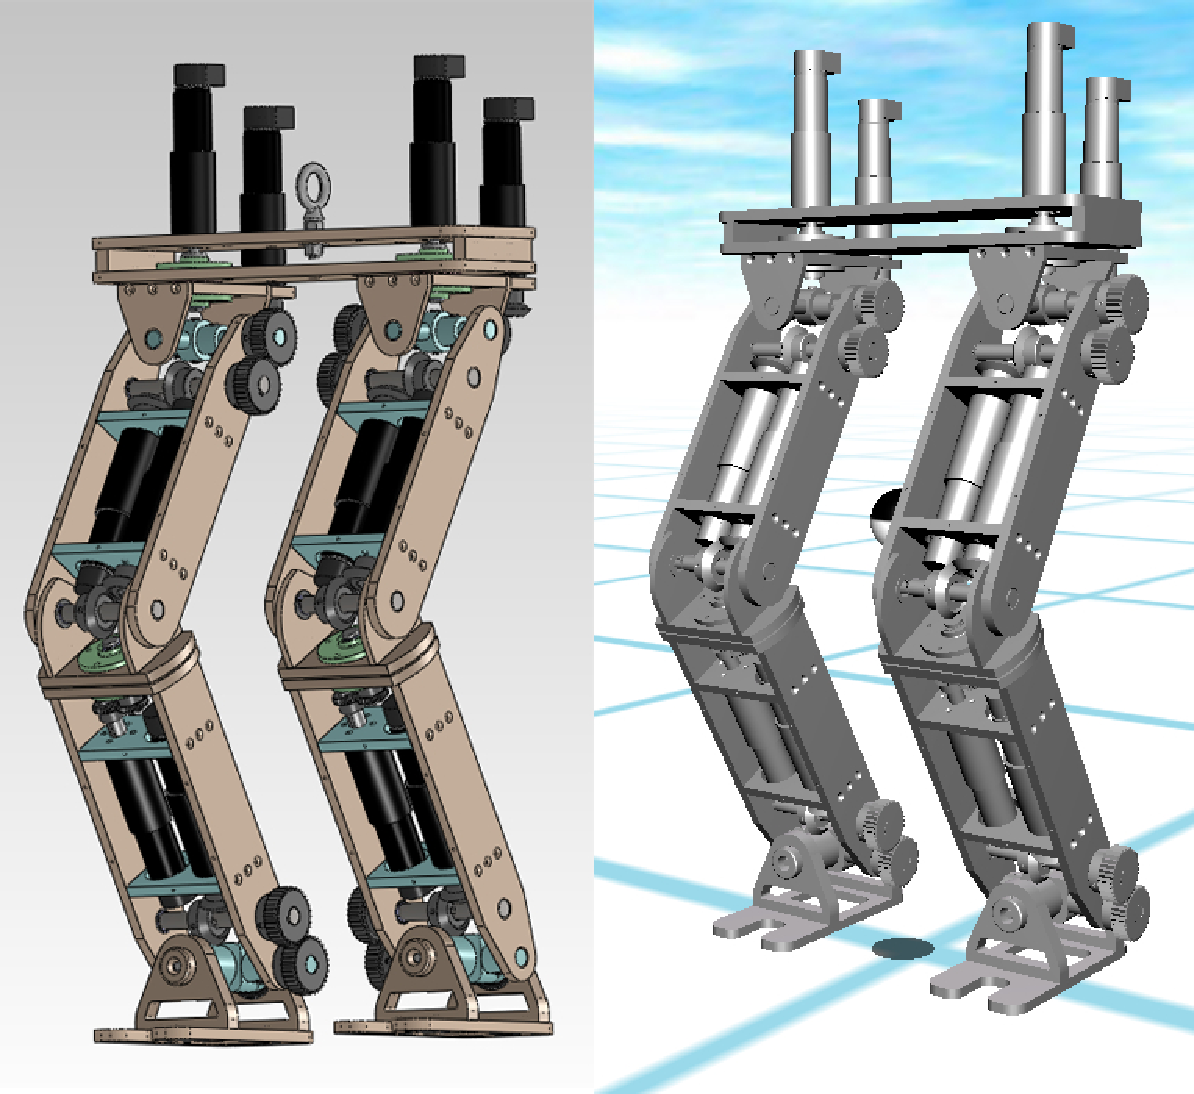
\includegraphics[scale=0.50]{fig/ch3/masterscene.pdf}
  	\caption{CAD master assembly shown on the left is used to automatically generate the meshes and scene file to recreate the visualization shown on the right.}
	\label{fig:masterscene}
\end{figure}

This approach allows the user to receive immediate visual feedback of the CAD model under the influence of control. This also allows the user to make changes to the mechanical design from visual observations (i.e. quick changes to improve joint limits).
% subsection visualization_model (end)

\subsection{Model Update} % (fold)
\label{sub:model_update}
The exporter add-in makes it possible to make changes to the mechanical design in CAD and generate the new kinematic and dynamic parameters immediately. After the initial model generation from CAD data, these new changes can be reflected back into the dynamic simulation by simply calling the update function. The update functionality also allows the user to specify the path to the previously generated physical model. The masked parameters on each link subsystem inside this model are simply updated with the new changes while the signal routing and everything else is left intact. The updated mesh files are loaded by the QUARC 3D viewer during the next simulation run.

This streamlines the iterative design process by allowing a user to export a system from the add-in and generate the CAD-equivalent physical/visual model in Simulink. The behaviour of the system can then be analyzed in dynamic simulations to revise the CAD design. Once the new changes are applied, the revised parameters are easily exported back into dynamic simulations for further analysis.
% subsection model_update (end)

% section model_generation (end)

\section{Case Study} % (fold)
\label{sec:case_study}

This toolchain was used to improve the initial design of the 14 DOF lower body humanoid robot\footnote{A video demonstration of the toolchain being used is available online at: \\ \url{https://ece.uwaterloo.ca/~dkulic/videos/Humanoids2012-480p.mp4}} discussed in Chapter \ref{cha:design}. The toolchain was used to quickly analyze the effects of design revisions (i.e. compare motor positioning) in simulation prior to manufacturing.

\subsection{Dynamic Simulations} % (fold)
\label{sub:dynamic_simulations}

The proposed toolchain was used during the design phase to estimate the torques at each joints for appropriate motor sizing. Changes to the mechanical design such as motor positioning and material of the links can significantly alter the torques required at some joints. In these situations it is useful to make incremental changes to analyze their impact on the system performance and immediately use this knowledge to tweak the design.

A common motion for humanoid robots is the bending of the knee and hip joints while a foot is swinging over during the gait cycle. During this phase, the motors at the hip joint must carry the overall weight of the leg below it. The choice of actuators on the leg plays a crucial role in its overall weight and as a result, also plays an important role in the torques required at these joints. Similarly, when the swing foot comes into contact with the ground, the knee joint absorbs a significant amount of torque so the motors must be sized appropriately.

\begin{figure}[!h]
	\begin{center}
	\subfigure{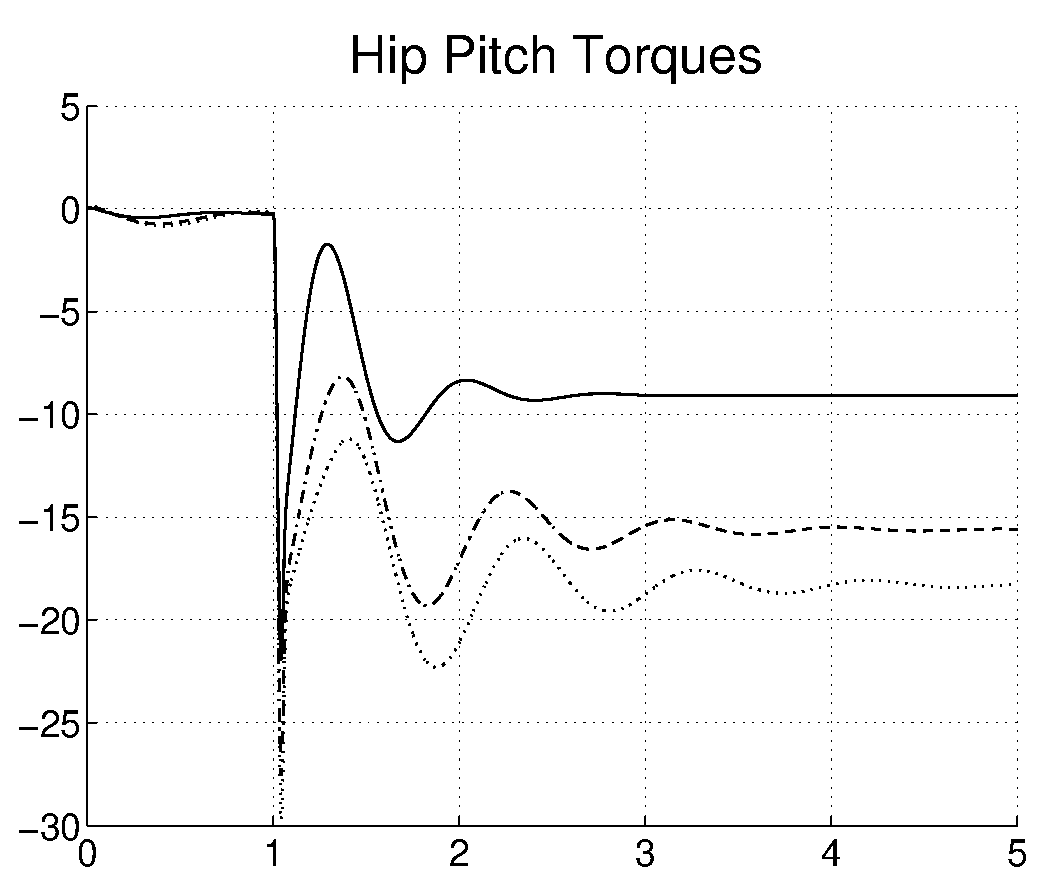
\includegraphics[scale=0.45]{fig/ch3/casestudy-hip.eps}}
	\subfigure{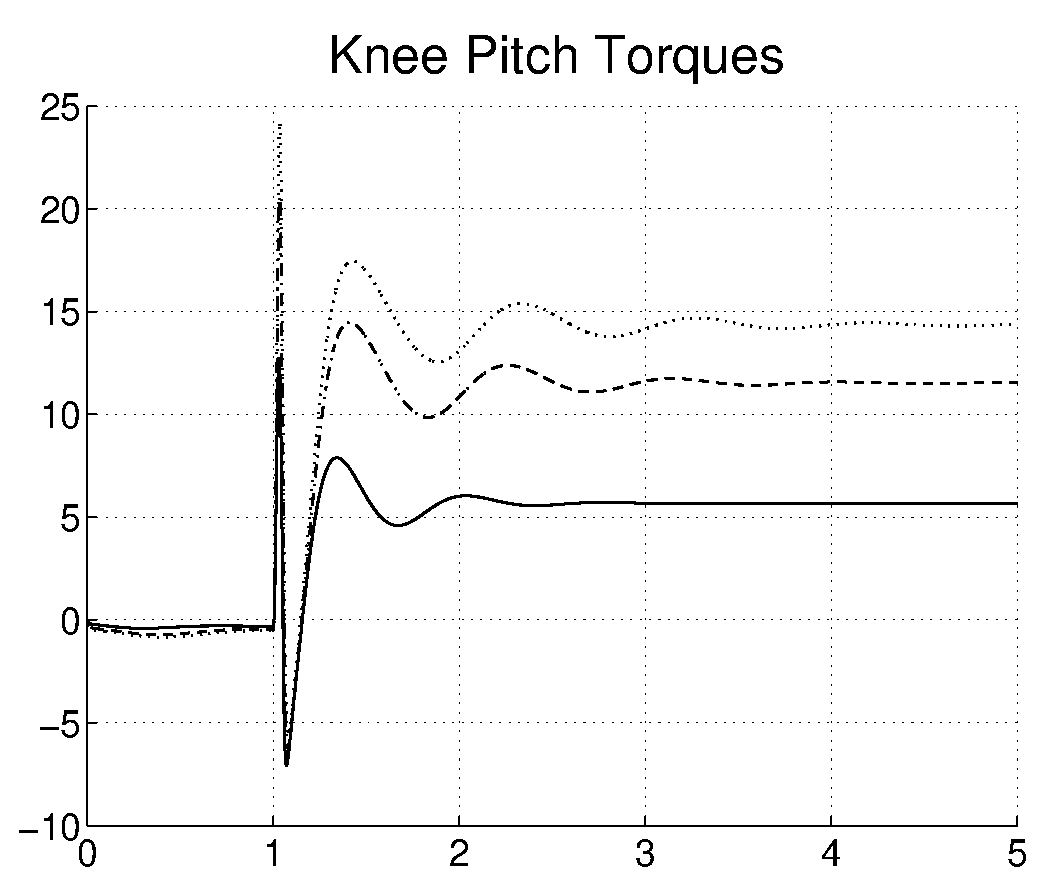
\includegraphics[scale=0.45]{fig/ch3/casestudy-knee.eps}}
	\end{center}
  	\caption{Hip and knee joint torque requirements while a leg is raised for different sets of motors at the joints.}
	\label{fig:casestudy}
\end{figure}

By using the toolchain, the user can maintain multiple configurations of the same mechanical design in CAD and export them for direct comparison with the dynamic simulator. Since the model is already defined, exporting each configuration takes less than a minute. The parameters of these configuration files can be used along with the model update feature to simulate each configuration and compare the results. In the case of bending the knee and hip joints, there may be several choices of motors which alter the system performance (due to large masses further down the leg). The torque profiles of each joint can be analyzed in the simulation (as shown in Figure \ref{fig:casestudy}) to select the most desirable configuration. The dotted and solid lines represent the heaviest and lightest motors, respectively. The dashed line represents the motor set with medium weight (between the heavy and light motors). The toolchain allows for fast incremental changes to revise the mechanical design and compare the torque requirements. 

% subsection dynamic_simulations (end)

\subsection{Visualization} % (fold)
\label{sub:visualization}
Additional meshes can also be added to the scene to serve as visual aids. For example, coordinate systems can be visualized during simulation by attaching arrow meshes to each link. Alternatively, common Simulink blocks can be used to determine if a particular joint is out of its limits and use the resulting signal to drive the colour of the mesh file (i.e. turn a link \emph{red} if the joint is out of its limits). A particularly useful visual aid for floating base multibody systems is the ability to see where the COM of the system is during simulation.  An additional mesh can be added to the scene driven by the COM calculation from forward kinematics at each time step. The use of this visual aid is shown in Figure  \ref{fig:visualcom}.

\begin{figure}[!h]
	\centering
    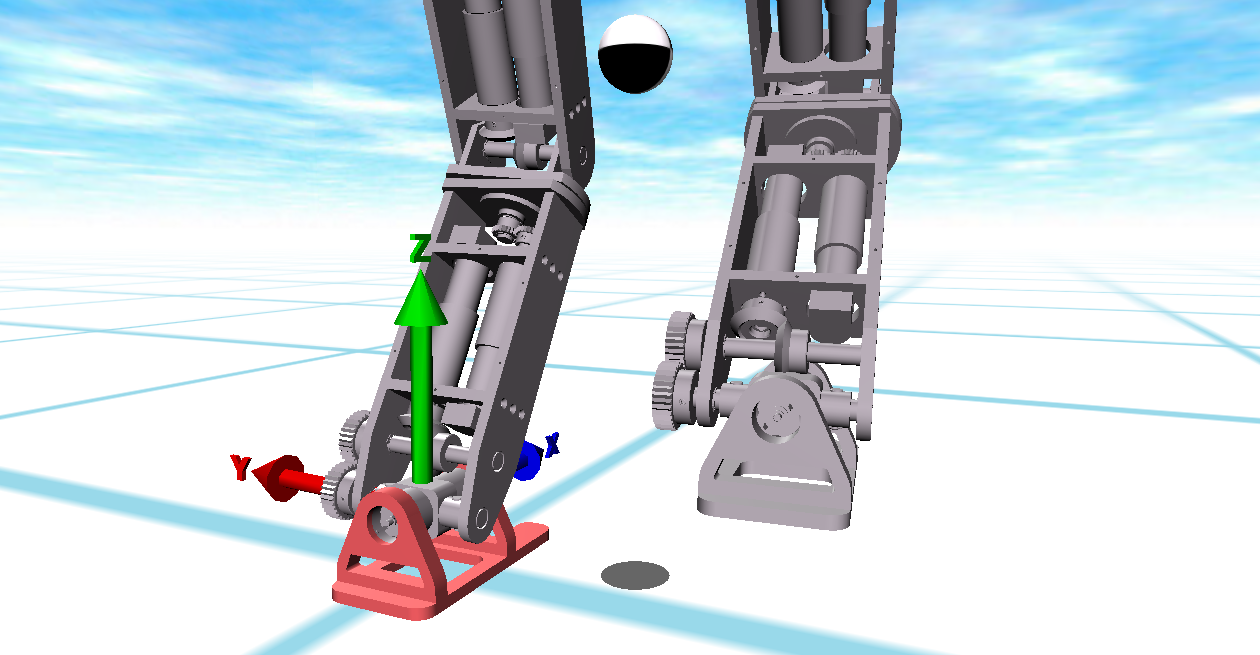
\includegraphics[scale=0.40]{fig/ch3/visualizecom.png}
  	\caption{Realtime visualization during simulations allows the user to get immediate visual feedback on important information like COM position.}
	\label{fig:visualcom}
\end{figure}

By having the visualization rendered in an external application, the proposed toolchain is capable of running simulations much faster than the built-in 3D viewing capabilities of SimMechanics. This increase in runtime speed is especially useful during the design phase where rapid iterations are common. The runtime for a 60s dynamic simulation\footnote{The simulations were executed on a standard PC available at the time of writing (2.4GHz Intel Core 2 Duo, 4 GB RAM).} at 1KHz \emph{with} visualization is compared in Table~\ref{tab:benchmark}. If the viewer is also being used to render the 3D mesh for each link through supplied VRML files, it takes much longer. In contrast, the proposed toolchain takes a fraction of the time for the exact same system to be simulated. The simultaneous visualization using the QUARC visualization toolset has little or no impact on the simulation speed. In fact, running the same dynamic simulation without the QUARC visualization toolset only reduces the overall runtime slightly.

\begin{table}[!h]
  \centering
  \caption{60s Dynamic Simulation Runtime}
    \begin{tabular}{lc}
    \addlinespace
    \toprule
    \textbf{Configuration} & \textbf{Runtime ($s$)}\\
    \midrule
    No Visualization 				& 47.50 	\\
    SimMechanics Visualization    	& 367	 	\\
    Proposed Toolset Visualization 	& 49 		\\
    \bottomrule
    \end{tabular}
  \label{tab:benchmark}
\end{table}

% subsection visualization (end)

% section case_study (end)

\section{Discussion} % (fold)
\label{sec:toolchain_discussion}
A streamlined toolchain was presented to enable rapid prototype development during the design and development phase of complex multibody systems. The toolchain exports a physical and visual representation of the CAD model which can be used to automatically generate dynamic simulations. After the initial model generation, subsequent exports simply update the physical model parameters and/or visualization blocks allowing for faster design iterations. 

The toolchain was used extensively during the design and development of the 14 DOF humanoid robot, demonstrating its usefulness in designing a physical robot. The simultaneous 3D visualization proved to be a tremendous benefit during the development of the 3D FPE theory that will be discussed in the following chapter. Through the use of visualization aids (i.e. for COM and ZMP position), it was very easy to analyze the behaviour of the system under control while the simulation was running. 
% section discussion (end)

% chapter toolchain (end)
